\documentclass[runningheads]{llncs}

\usepackage[T1]{fontenc}
\usepackage[utf8]{inputenc}
\usepackage{graphicx}
\usepackage{booktabs}
\usepackage{multirow}
\usepackage{url}
\usepackage{xspace}
\usepackage{amsmath}
\usepackage{tikz}
\usetikzlibrary{shapes.geometric,positioning,arrows.meta}

\newcommand{\method}{SchemaShield-Lite\xspace}

\begin{document}

\title{Tool Calling Under Interface Drift: A Non-Oracle Study of Validation and Repair}
\titlerunning{Tool Calling Under Interface Drift}

\author{Anonymous Authors}
\authorrunning{Anonymous Authors}
\institute{Draft prepared for NGEN-AI 2026}

\maketitle

\begin{abstract}
Tool-calling language models rely heavily on surface-form tool interfaces, including
descriptions, parameter names, and candidate tool sets. In realistic deployments,
these interfaces drift after release even when the underlying tool semantics remain
unchanged. We study this problem as \emph{interface drift} and evaluate a lightweight
training-free mitigation, \method, built from validation, candidate-set retry,
and one-shot repair. Our primary protocol is \emph{non-oracle}: the repair stage
never receives the benchmark gold tool identity, and missing tool names are handled
by retrying over only the visible candidate tools. On Qwen3.5-9B, this protocol
raises DICE-300 accuracy from $0.717$ under drift to $0.813$ after repair and
BFCL-200 accuracy from $0.580$ to $0.805$, with zero repair harms on the
originally-correct slice in both benchmarks. A naive-retry baseline reaches only
$0.707$ on DICE and $0.585$ on BFCL, showing that the gains do not come from a
second attempt alone. On our DICE-300 Qwen3.5-9B ablation, candidate-set drift
dominates the base damage: description-only and schema-only drift cause $< 1.5$ point
degradations on DICE, while distractor tools account for nearly all of the drop.
In the non-oracle setting, missing tool names are a major bottleneck; adding a
candidate-set retry reduces unresolved repair targets from $35$ to $15$ on DICE
and from $34$ to $9$ on BFCL. Additional oracle-constrained sweeps across other
models serve as upper bounds and error-analysis context, but we treat the
non-oracle Qwen3.5-9B results as the primary deployment-facing evidence.
\keywords{tool calling \and language models \and robustness \and interface drift \and repair}
\end{abstract}

\section{Introduction}
Modern language-model agents increasingly depend on external tools for retrieval,
execution, planning, and actuation. In practice, however, tool use is mediated
entirely through text: tool descriptions, parameter schemas, enum values, and
candidate tool lists. Recent work shows that these interface details strongly affect
tool selection and argument generation
even when the tool semantics are unchanged \cite{guo2026rewrite,faghih2025gaming}.
This creates a deployment problem: tool interfaces drift over time as developers
rename parameters, revise descriptions, add examples, or expand candidate tool sets.

We study this problem as \emph{interface drift}: benign, semantics-preserving
changes to tool interfaces that occur after deployment. Our goal is not to train a
new tool-calling model, but to quantify drift sensitivity and test whether a compact
inference-time repair layer can recover reliability without retraining.

We instantiate drift with three deployment-motivated synthetic perturbations: (i) stale description
examples that mention legacy field names, (ii) schema renaming, and (iii) distractor
tools. Our primary evaluation uses Qwen3.5-9B on a 300-example DICE-BENCH slice
\cite{jang2025dicebench} and a 200-example BFCL slice \cite{bfcl2024} under a
deployment-realistic non-oracle repair protocol. In that protocol, validation runs
against the visible tool selected by the model; if the model omits the tool name, a
candidate-set retry over the visible tools resolves a concrete target before repair.
We also retain earlier oracle-constrained sweeps on additional open models as
upper-bound context and for secondary analyses.

This paper makes four empirical contributions that substantially revise the
narrative of prior interface-drift work:

\begin{enumerate}
\item \textbf{Non-oracle inference-time repair recovers drift-induced failures
with zero harms on the primary model.} On Qwen3.5-9B, \method raises DICE-300
accuracy from $0.717$ to $0.813$ and BFCL-200 accuracy from $0.580$ to $0.805$,
while preserving zero repair harms on the originally-correct slice in both
benchmarks.

\item \textbf{Naive retry does not explain the gains.} On DICE-300, naive retry
reaches $0.707$ versus repaired $0.813$; on BFCL, $0.585$ versus $0.805$. A second
attempt alone therefore cannot explain the recovery.

\item \textbf{Candidate-set drift dominates the damage on our primary-model ablation.}
Under description-only drift or schema-only drift, Qwen3.5-9B accuracy drops by just
$0.013$ and $0.007$ points respectively. Adding distractor tools causes a $0.047$
drop, matching the full combined drift.

\item \textbf{Missing tool names are the main non-oracle bottleneck, and a
candidate-set retry largely closes that gap.} In the non-oracle setting, adding a
candidate-set retry improves repaired accuracy from $0.780$ to $0.813$ on DICE and
from $0.725$ to $0.805$ on BFCL, while reducing unresolved repair targets from $35$
to $15$ and from $34$ to $9$ respectively.
\end{enumerate}

\section{Related Work}
Recent work has established that tool interfaces are not neutral wrappers around
tool use; they are part of the learning and inference problem itself.
Guo et al.~\cite{guo2026rewrite} show that rewriting tool descriptions can
substantially improve agent reliability, especially when candidate tool sets are
large. Faghih et al.~\cite{faghih2025gaming} show the opposite direction:
small edits to tool descriptions can dramatically shift tool preference, exposing a
fragility in description-mediated tool use.

Several recent papers study robustness and recovery in tool-use systems.
Zhang et al.~\cite{zhang2026fission} show that execution-error recovery remains a
major weakness, particularly for smaller models, and propose RL-based training to
improve it. Our setting is narrower and more deployment-oriented: we target
inference-time robustness under interface drift rather than post-training
optimization.

Benchmark work has also highlighted that realistic function calling is still far from
solved. ComplexFuncBench introduces multi-step and constrained long-context function
calling \cite{zhong2025complexfuncbench}, while DICE-BENCH focuses on multi-round,
multi-party dialogues with tool-related information dispersed across conversation
turns \cite{jang2025dicebench}. We evaluate on both DICE-BENCH and the Berkeley
Function Calling Leaderboard (BFCL) \cite{bfcl2024} because they capture
complementary settings: DICE-BENCH exercises conversational multi-turn dialogues,
while BFCL tests single-turn tool calls across diverse APIs.

Broader tool-use work has focused on scaling tool coverage and agent behavior rather
than on post-deployment interface drift. ToolLLM and ToolBench study large-scale
API-use training and evaluation across thousands of real-world tools
\cite{qin2023toolllm}, while Gorilla emphasizes retrieval and function selection over
large API collections \cite{patil2023gorilla}. Agent frameworks such as ReAct and
Reflexion show that multi-step reasoning, action, and self-correction can materially
improve tool-using systems \cite{yao2022react,shinn2023reflexion}. Our setting is
narrower: we isolate a deployment-time robustness problem in which tool semantics are
fixed but interface surface form changes after release.

Compared with dataset-generation work such as APIGen \cite{liu2024apigen}, our
objective is different. We do not create new large-scale tool-calling training data.
Instead, we evaluate whether a lightweight repair layer can stabilize existing models
against a specific class of post-deployment failures.

\section{Problem Formulation}
Let a tool be represented by an interface
$I = (d, s, C)$, where $d$ is the natural-language description, $s$ is the argument
schema, and $C$ is the candidate tool set shown to the model. The underlying tool
semantics are assumed fixed. An \emph{interface drift} operator $\Delta$ maps $I$ to
a new interface $\Delta(I)$ that preserves tool semantics but perturbs surface form.

We study three drift types:
\begin{itemize}
\item \textbf{Description drift}: add stale or legacy examples to the description that
refer to older field names.
\item \textbf{Schema drift}: rename parameters while preserving semantics.
\item \textbf{Candidate-set drift}: add distractor tools with overlapping descriptions.
\end{itemize}

Given user context $x$, tool interface $I$, and model $M$, the base system outputs a
tool call $y = M(x, I)$. We evaluate three stages:
\begin{enumerate}
\item \textbf{Original}: inference on the original tool interface.
\item \textbf{Drifted}: inference on the drifted interface $\Delta(I)$.
\item \textbf{Repaired}: inference-time repair of an invalid or incomplete drifted call.
\end{enumerate}

Our central question is whether an inference-time repair layer can recover the
performance lost from Original to Drifted without harming examples that were already
correct.

\section{Method}
\label{sec:method}
\subsection{\method}
\method is a lightweight inference-time robustness layer with three parts.
Figure~\ref{fig:pipeline} sketches the full pipeline.

\begin{figure}[t]
\centering
\resizebox{\linewidth}{!}{%
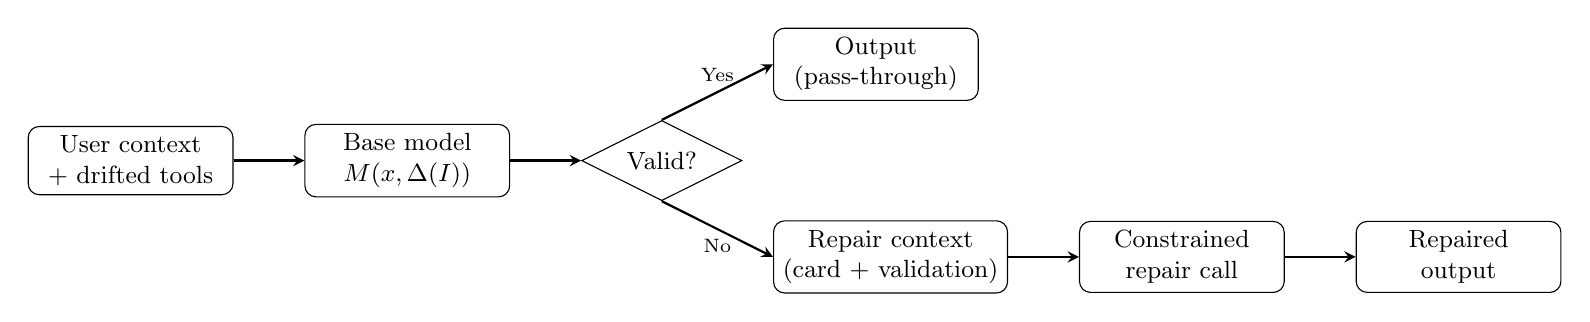
\begin{tikzpicture}[
    node distance=0.9cm and 0.9cm,
    box/.style={draw, rounded corners, minimum width=2.6cm, minimum height=0.8cm, align=center, font=\small},
    decision/.style={draw, diamond, aspect=2, minimum width=1.4cm, align=center, font=\small},
    arrow/.style={->, >=stealth, thick},
]
\node[box] (input) {User context\\+ drifted tools};
\node[box, right=of input] (model) {Base model\\$M(x, \Delta(I))$};
\node[decision, right=of model] (valid) {Valid?};
\node[box, above right=0.5cm and 0.9cm of valid] (pass) {Output\\(pass-through)};
\node[box, below right=0.5cm and 0.9cm of valid] (repair) {Repair context\\(card + validation)};
\node[box, right=of repair] (repairmodel) {Constrained\\repair call};
\node[box, right=of repairmodel] (output) {Repaired\\output};

\draw[arrow] (input) -- (model);
\draw[arrow] (model) -- (valid);
\draw[arrow] (valid.north) -- node[above, font=\scriptsize] {Yes} (pass.west);
\draw[arrow] (valid.south) -- node[below, font=\scriptsize] {No} (repair.west);
\draw[arrow] (repair) -- (repairmodel);
\draw[arrow] (repairmodel) -- (output);
\end{tikzpicture}
}
\caption{\method pipeline. The base model receives user context and drifted tool
definitions. If the emitted tool call fails validation, a repair call is issued
with structured validation errors. In the primary non-oracle protocol, missing tool
names are first resolved by retrying over the visible candidate tools; once a
visible target tool is resolved, a repair step may be constrained to that selected
tool where provider support allows.}
\label{fig:pipeline}
\end{figure}


\paragraph{Canonical tool card.}
Each tool is rendered into a compact canonical form containing the tool name,
description, required fields, and field-level type information. This normalizes
interface presentation across tools and emphasizes current field names.

\paragraph{Validation.}
After the base model emits a tool call, a validator checks tool name, required
fields, and argument structure. Validation produces a structured error report rather
than a binary failure signal.

\paragraph{One-shot repair.}
If the drifted call is invalid, the model receives a repair prompt containing the
task context, canonical tool card, invalid call, and validation errors. In the
primary non-oracle protocol, repair proceeds in two stages. If the base call names
a visible tool, validation runs against that tool and a constrained repair call is
issued for that same visible tool. If the base call omits the tool name, we first
run a candidate-set retry over the visible tools to produce a concrete tool call;
once a visible tool is resolved, a second repair call may be constrained to that
selected tool. Where provider support allows it, this second step uses
\emph{forced-tool repair}; otherwise we fall back to unconstrained tool calling or
JSON repair.

As our component ablation in Section~\ref{sec:component-ablation} shows, it is the
combination of structured validation errors and tool-constrained repair that does
the heavy lifting once a visible target tool has been resolved. The canonical card
is useful at the initial prediction step as drift-prevention prompting, but
contributes negligibly to repair-stage recovery in our oracle-constrained
upper-bound ablations.

\subsection{Repair Prompting Details}
Two implementation details turned out to matter materially:
\begin{itemize}
\item The repair prompt explicitly instructs the model to infer all required fields
from the dialogue even when the invalid call is empty.
\item When the invalid call omits the tool name, a candidate-set retry over the
visible tools is needed before tool-constrained repair can fire.
\item The repair stage uses a larger token budget than the base prediction stage.
Raising repair capacity from the earlier default to $512$ tokens fixed truncated
repair outputs on longer DICE dialogues.
\end{itemize}

\section{Experimental Setup}
\subsection{Benchmarks and Data Slices}
We evaluate on two benchmarks. For DICE-BENCH \cite{jang2025dicebench}, we use a
300-example subset drawn from single-function round-1 dialogues (allowing duplicate
functions to reach sufficient scale). For BFCL \cite{bfcl2024}, we use a 200-example
subset drawn in equal parts from four categories: simple Python, multiple-function,
live-simple, and live-multiple.

\subsection{Models}
We evaluate four open instruction-tuned models accessed via OpenRouter:

\begin{itemize}
\item \textbf{Qwen3.5-9B}: our primary model.
\item \textbf{Qwen3.5-35B-A3B}: larger MoE variant.
\item \textbf{Llama-4-Scout}: Meta's 2025 open model.
\item \textbf{Mistral-Small-3.2-24B}: recent Mistral dense model.
\end{itemize}

All experiments use temperature $0.0$ for deterministic-style evaluation.

\subsection{Drift Configurations}
For DICE main runs, we use \emph{mild} severity: two description modes
(\texttt{legacy\_example}, \texttt{marketing}), two schema modes
(\texttt{rename\_parameters}, \texttt{reorder\_parameters}), and one distractor
tool. For BFCL we use \emph{medium} severity: three description modes, three schema
modes, and three distractors, reflecting a more aggressive drift scenario. These
operators are author-designed and deployment-motivated rather than mined from real
API changelogs; we return to that limitation in Section~8.

\subsection{Repair Protocols}
We use two repair protocols. Our \emph{primary} protocol is non-oracle and is the
main evidence in this paper: the validator checks the model-selected visible tool,
and when the model omits the tool name, a candidate-set retry over only the visible
tools resolves a target before repair. For broader model coverage and component
ablations, we also retain earlier \emph{oracle-constrained upper-bound} sweeps in
which the repair stage is given the benchmark target tool. These upper-bound runs
remain useful for cross-model context and ablation, but they are not the paper's
deployment-facing evidence.

\subsection{Metrics}
We report:
\begin{itemize}
\item \textbf{Original score}: accuracy on the unmodified interface.
\item \textbf{Drifted score}: accuracy under interface drift.
\item \textbf{Repaired score}: accuracy after one-shot repair.
\item \textbf{Naive retry score}: accuracy under a second identical drifted call
(no canonical card, no validation feedback). This baseline isolates the value of
simply retrying.
\item \textbf{Originally-correct slice}: the subset of examples that the model solves
correctly before drift. This slice isolates \emph{true drift harm} from baseline
errors.
\item \textbf{Repair recoveries}: drift-induced failures recovered by repair.
\item \textbf{Repair harms}: drifted-correct examples broken by repair.
\item \textbf{Repair trigger rate}: fraction of examples for which the validator
invokes the repair step.
\end{itemize}

\section{Results}
\subsection{Primary Non-Oracle Results and Oracle Upper Bounds}
Table~\ref{tab:main-results} summarizes our primary non-oracle Qwen3.5-9B results
on DICE-300 and BFCL-200, together with earlier oracle-constrained upper bounds for
reference. Under the non-oracle candidate-retry protocol, \method improves over the
drifted baseline on both benchmarks with \emph{zero repair harms} on the
originally-correct slice.

\begin{table}[t]
\caption{Primary non-oracle Qwen3.5-9B results on DICE-300 and BFCL-200, with
oracle-constrained upper bounds for reference. Brackets give 95\% bootstrap
confidence intervals (seed~42). OC = originally-correct count;
Rec = recoveries on drift-induced failures; Harms = repair harms on
originally-correct slice; Trig\% = repair trigger rate.}
\label{tab:main-results}
\centering
\scriptsize
\setlength{\tabcolsep}{3.5pt}
\resizebox{\linewidth}{!}{%
\begin{tabular}{llccccccc}
\toprule
Benchmark & Protocol & Orig. [95\% CI] & Drift. [95\% CI] & Repair [95\% CI] & OC & Rec/Miss & Harms & Trig\% \\
\midrule
\multirow{2}{*}{DICE-300}
& Non-oracle + candidate retry & 0.757 [0.70, 0.80] & 0.717 [0.67, 0.77] & \textbf{0.813 [0.77, 0.86]} & 227 & 19/22 & 0 & 16.0 \\
& Oracle upper bound           & 0.750 [0.70, 0.80] & 0.713 [0.66, 0.76] & \textbf{0.827 [0.79, 0.87]} & 225 & 17/18 & 0 & 21.0 \\
\midrule
\multirow{2}{*}{BFCL-200}
& Non-oracle + candidate retry & 0.790 [0.74, 0.84] & 0.580 [0.51, 0.65] & \textbf{0.805 [0.75, 0.86]} & 158 & 33/45 & 0 & 32.0 \\
& Oracle upper bound           & 0.790 [0.74, 0.84] & 0.640 [0.58, 0.71] & \textbf{0.795 [0.74, 0.85]} & 158 & 23/35 & 0 & 31.0 \\
\bottomrule
\end{tabular}
}
\end{table}

\begin{figure}[t]
\centering
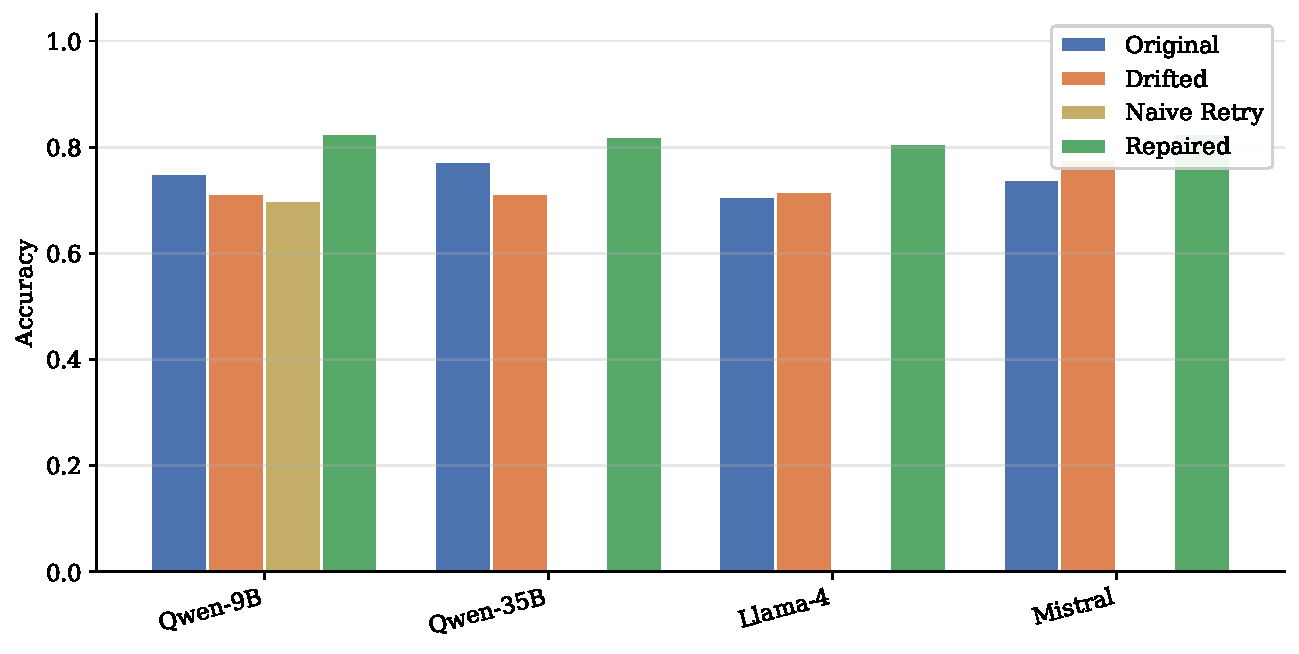
\includegraphics[width=0.9\linewidth]{figures/accuracy_bars.pdf}
\caption{Oracle-constrained upper-bound DICE sweep across the four evaluated
models. We retain these runs as secondary cross-model context; the paper's primary
deployment-facing evidence is the non-oracle Qwen3.5-9B protocol in
Table~\ref{tab:main-results}.}
\label{fig:accuracy-bars}
\end{figure}

The primary non-oracle results are strong on both benchmarks. On DICE-300, repair
improves Qwen3.5-9B from $0.717$ to $0.813$ and recovers $19/22$ drift-induced
failures on the originally-correct slice. On BFCL-200, repair improves from $0.580$
to $0.805$ and recovers $33/45$ drift-induced failures. The remaining gap to the
oracle upper bound is small on DICE ($0.813$ vs $0.827$), and on BFCL the final
non-oracle candidate-retry run slightly exceeds the earlier oracle-style run
($0.805$ vs $0.795$).

We therefore focus our interpretation on the large repaired-vs-drifted gaps, not on
small differences between nearby runs. The bootstrap intervals in
Table~\ref{tab:main-results} support the main claim that structured repair helps,
but they do not justify strong claims about minor oracle-vs-non-oracle differences.
Paired exact McNemar tests on the final non-oracle runs also support the main
repair effect: repaired beats drifted with $p=3.7\times 10^{-9}$ on DICE and
$p=5.7\times 10^{-14}$ on BFCL.

The candidate-set retry is load-bearing in the non-oracle setting. Relative to an
earlier non-oracle run that simply skipped unresolved tool names, candidate retry
raises repaired accuracy from $0.780$ to $0.813$ on DICE and from $0.725$ to
$0.805$ on BFCL, while reducing unresolved repair targets from $35$ to $15$ and
from $34$ to $9$ respectively.

\paragraph{Repair cost overhead.}
On the final non-oracle Qwen3.5-9B runs, \method triggers repair on $48/300$
examples ($16.0\%$) in DICE and $64/200$ examples ($32.0\%$) in BFCL. Total repair
tokens are $103{,}221$ against $316{,}185$ drifted tokens on DICE ($32.6\%$
relative overhead) and $154{,}249$ against $327{,}289$ drifted tokens on BFCL
($47.1\%$ relative overhead). Because repair is gated by validation, this overhead
is paid only when the drifted call is invalid or incomplete. On a refreshed
BFCL-200 live rerun of the same non-oracle protocol with latency instrumentation,
average original-call latency is $8.8$s, average drifted-call latency is $9.3$s,
and average repair-call latency when repair fires is $13.0$s. With a $27.0\%$
repair trigger rate on that rerun, this corresponds to roughly $3.5$s expected
added latency per example.

\subsection{Naive Retry Does Not Explain the Gains}
\label{sec:naive-retry}
A first-order alternative explanation is that repair works simply because the model
gets a second attempt. We test this by running a \emph{naive retry} call that uses
the same drifted tools but without the canonical card or the validation error
report. Table~\ref{tab:naive-retry} shows that naive retry remains far below
structured repair: $0.707$ vs $0.813$ on DICE and $0.585$ vs $0.805$ on BFCL.
Naive retry is therefore insufficient to explain the gains, even though it is nearly
flat with drifted performance on BFCL. The paired repaired-vs-naive contrast is
also highly significant on both benchmarks (exact McNemar $p=4.1\times 10^{-9}$
on DICE; $p=1.1\times 10^{-13}$ on BFCL).

\begin{table}[t]
\caption{Naive retry vs the primary non-oracle \method protocol on Qwen3.5-9B.}
\label{tab:naive-retry}
\centering
\small
\begin{tabular}{lcccc}
\toprule
Benchmark & Drifted & Naive Retry & \method & $\Delta$ over Drifted \\
\midrule
DICE-300   & 0.717 & 0.707 & \textbf{0.813} & $+0.097$ \\
BFCL-200   & 0.580 & 0.585 & \textbf{0.805} & $+0.225$ \\
\bottomrule
\end{tabular}
\end{table}

\subsection{Drift-Type Ablation: Candidate-Set Drift Dominates}
\label{sec:drift-ablation}
Table~\ref{tab:drift-ablation} decomposes the drift pipeline into its three
components and evaluates each in isolation at DICE-300 on Qwen3.5-9B. Description
drift alone causes only a $0.013$ point accuracy drop. Schema drift alone causes
only $0.007$. By contrast, candidate-set drift (adding a distractor tool) causes a
$0.047$ drop---matching the full combined drift scenario ($0.050$). Because this
ablation is about where the damage comes from, the main interpretation rests on the
Original-to-Drifted delta rather than the repair column.

\begin{table}[t]
\caption{Drift-type ablation on DICE-300 with Qwen3.5-9B. Orig./Drift. scores come
from the base model; Repair scores are from the oracle-constrained upper-bound
repair protocol.}
\label{tab:drift-ablation}
\centering
\small
\begin{tabular}{lcccr}
\toprule
Drift type & Orig. & Drift. & Repair & Drift Drop \\
\midrule
Description only     & 0.760 & 0.747 & 0.813 & $-0.013$ \\
Schema only          & 0.767 & 0.760 & 0.830 & $-0.007$ \\
Candidate-set only   & 0.757 & 0.710 & 0.830 & $-0.047$ \\
\textbf{All combined}& 0.763 & 0.713 & 0.823 & $-0.050$ \\
\bottomrule
\end{tabular}
\end{table}

\begin{figure}[t]
\centering
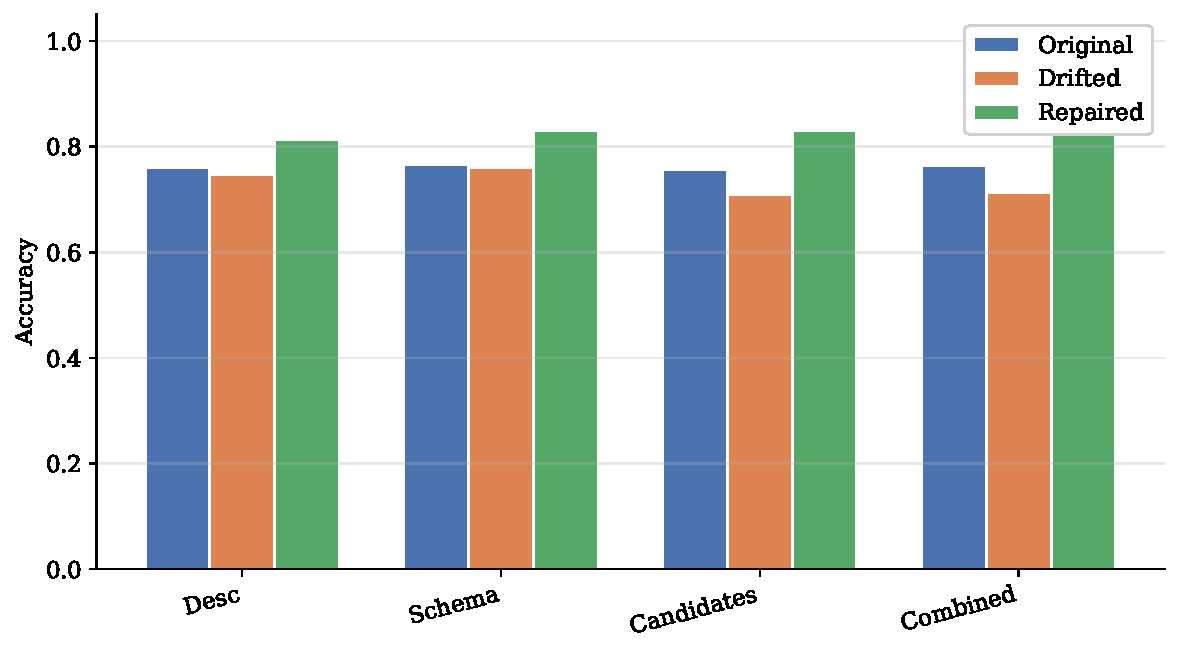
\includegraphics[width=0.82\linewidth]{figures/drift_ablation.pdf}
\caption{Drift-type ablation on DICE-300 with Qwen3.5-9B. Description-only and
schema-only drift cause negligible accuracy drops. Adding distractor tools
reproduces essentially all of the damage of the full combined drift.}
\label{fig:drift-ablation}
\end{figure}

This result qualifies a common framing in the interface-drift literature. On this
Qwen3.5-9B DICE-300 ablation, minor description rewording and
semantics-preserving parameter renames do not meaningfully degrade accuracy---the
model is evidently robust to this class of surface perturbation. The observed
failure mode is \emph{candidate-set confusion}: when a distractor tool with an
overlapping description is added to the candidate set, tool selection degrades.
This has implications for deployment-time monitoring: teams should prioritize
tracking tool-catalog growth over monitoring description or schema revisions.

\subsection{Upper-Bound Component Ablation: Validation, Not Canonical Card, Drives Recovery}
\label{sec:component-ablation}
To isolate which parts of the repair stack matter once a target tool has already
been resolved, Table~\ref{tab:component-ablation} evaluates three variants of
\method in an oracle-constrained upper-bound setting on both DICE-300 and BFCL-200
with Qwen3.5-9B: (i) canonical card only, where the card is prepended to the
initial prompt but no validation/repair is applied; (ii) validation-plus-retry,
which uses validation errors in a repair prompt but omits the canonical tool card
from the repair context; and (iii) full \method (card + validation + repair).

\begin{table}[t]
\caption{Oracle-constrained upper-bound component ablation on DICE-300 and
BFCL-200 with Qwen3.5-9B. BFCL uses medium-severity drift, DICE uses mild.}
\label{tab:component-ablation}
\centering
\small
\begin{tabular}{llcccccc}
\toprule
Benchmark & Variant & Drift. & Repair & Rec/Miss & Harms & Trig\% \\
\midrule
\multirow{3}{*}{DICE-300}
& Canonical card only            & 0.770 & 0.770 & 0/9   & 0 & 0.0 \\
& Validation + retry (no card)   & 0.730 & 0.830 & 16/17 & 0 & 20.0 \\
& \textbf{Full \method}          & 0.713 & \textbf{0.827} & 17/18 & 0 & 21.0 \\
\midrule
\multirow{3}{*}{BFCL-200}
& Canonical card only            & 0.810 & 0.810 & 0/11  & 0 & 0.0 \\
& Validation + retry (no card)   & 0.645 & \textbf{0.820} & 26/34 & 0 & 29.5 \\
& Full \method                   & 0.640 & 0.795 & 23/35 & 0 & 31.0 \\
\bottomrule
\end{tabular}
\end{table}

Within this oracle-constrained setting, the BFCL rows confirm and \emph{strengthen}
the DICE finding in three ways.
First, the canonical card at initial-prediction time provides even stronger
drift prevention on BFCL than on DICE: the base drifted score of $0.640$ jumps
to $0.810$---a $17.0$-point drift-prevention effect. Second, the card-only
configuration still never triggers the validator and recovers zero
drift-induced failures, because its valid-but-imperfect outputs pass schema
checking without entering the repair path. Third, validation-plus-retry
without the canonical card at repair time reaches a \emph{higher} repaired
accuracy on BFCL than the full pipeline ($0.820$ vs $0.795$, and $26/34$
recoveries vs $23/35$), matching the pattern observed on DICE where
validation-only nearly ties the full pipeline.

Taken together across both benchmarks, these upper-bound numbers localize the
load-bearing component of \method to the validation error feedback loop
combined with tool-constrained repair, not the canonical tool card presented at
repair time. The card earns its keep as \emph{drift-prevention prompting}
at the initial prediction step---where BFCL shows it can dominate the
remaining drift damage---but can be dropped from the repair prompt without
hurting recovery once the target tool has already been resolved.

\subsection{Error Analysis}
\label{sec:error-analysis}
Across the oracle-constrained DICE upper-bound sweeps, all repair harms are zero.
However, not every drift miss is recovered. On Qwen3.5-35B, repair recovers $20$ of
$25$ drift misses; on Llama-4-Scout, $12$ of $16$; on Mistral, $8$ of $12$. We
manually inspected every unrecovered case on these three runs and classified them
against the gold call.

The pattern is consistent across models: nearly all unrecovered examples
involve the repair call selecting the correct tool with well-formed arguments
whose string values disagree with gold only by formatting or paraphrase. On
Qwen3.5-35B ($5$ unrecovered), these include one strict whitespace/punctuation
difference (``\texttt{the quick brown fox\ldots}'' vs
``\texttt{The quick brown fox\ldots.}'') and three enum-format or
paraphrase-level mismatches (e.g.\ \texttt{regular\_season} vs
\texttt{regular season}, \texttt{the office} vs \texttt{Office}); a single
genuine failure has an empty arguments object after repair. On Llama-4-Scout
($4$ unrecovered), all four are format-level: \texttt{ISO}-prefixed dates
vs two-field dates (e.g.\ \texttt{2023-11-10} vs \texttt{11-10}), or JSON
with quoted-number string values rather than numeric literals. On Mistral-24B
($4$ unrecovered), the misses include near-synonym topics (\texttt{inspirational}
vs \texttt{inspiration}, \texttt{AI} vs \texttt{artificial intelligence},
\texttt{Google} vs \texttt{GOOGL}) and one wrong numeric amount. Across
13~unrecovered cases in total, only $2$ are genuine inference failures
(empty arguments and one wrong value); the remaining $11$ are strict-match
artifacts rather than true drift failures. The practical implication is that
the paper's reported recovery rates are a lower bound: a lenient evaluator
would count most of the unrecovered cases as correct.

On the primary non-oracle Qwen3.5-9B runs, repair improves over the drifted call on
$29$ DICE examples and $45$ BFCL examples in total. Not all of these are pure drift
recovery: $10$ of the DICE gains and $12$ of the BFCL gains are baseline-error
patching on examples the base model already missed before drift. This side effect is
useful in deployment, but it reinforces the need to separate drift recovery from
general post-hoc correction in the paper's reporting.

Mistral-24B exhibits an unusual pattern: its drifted score ($0.777$) is
slightly higher than its original score ($0.740$). Inspection of the $23$
examples where Mistral's original call misses but the drifted call matches
shows that almost none of them involve the model recovering extra information
from the drifted description. Instead, $15/23$ are strict-match artifacts on
the original call: formatting differences in the value (\texttt{apple} vs
\texttt{apples}, \texttt{bread, eggs, cheese} vs \texttt{bread,eggs,cheese},
\texttt{https://wikipedia.org/} vs \texttt{https://wikipedia.org}), and only
a handful reflect the model missing a required field in the original call
($4/23$) or choosing a wrong tool name ($4/23$). The drifted call happens to
land in the tokenization bucket that the scorer accepts, pushing the scored
accuracy slightly above the original. We therefore read the Mistral
``drift~$>$~original'' effect as scorer noise rather than as evidence that
description drift helps Mistral, and revise the original speculation
accordingly.

\section{Discussion}
Our results support three narrower conclusions than the original \method framing
suggested. First, non-oracle inference-time repair is a viable robustness layer for
tool-calling systems under interface drift: on Qwen3.5-9B it improves over drifted
performance on both DICE and BFCL while preserving zero harms on the
originally-correct slice. Second, the main non-oracle bottleneck is missing tool
names; a candidate-set retry over the visible tools closes much of the gap to the
oracle upper bound. Third, the \emph{target} of robustness work is candidate-set
drift rather than description or schema drift.

Together these findings simplify the deployment picture. A practitioner does not
need a heavy per-tool canonicalization pipeline; a visible-tool validator, a
candidate-set retry for missing tool names, and a constrained repair call once a
tool is resolved already recover most of the damage we observe. And the monitoring
story is clearer: the first-order cause of post-deployment tool-calling regressions
is likely tool-catalog expansion, not description or parameter rename churn.

\section{Limitations}
Several limitations remain. First, our primary non-oracle deployment-facing
evaluation is currently on a single model, Qwen3.5-9B; the broader multi-model
results retained in the paper are oracle-constrained upper bounds rather than
full non-oracle replications. Second, the BFCL evaluation still covers only two
models due to API-cost constraints. Third, our drift operators focus on stale
descriptions, renamed fields, and distractors; other forms of interface drift
(for example, type narrowing, enum replacement, or multi-tool refactors) remain
untested, and the perturbations are author-designed rather than mined from real
API evolution logs. Fourth, evaluation uses hosted inference and so may incorporate
provider-specific tool-calling behavior. Fifth, the ``repair $>$ original''
effect indicates that \method is also patching baseline failures---useful in
deployment, but a complication for clean attribution to drift recovery
specifically. Sixth, strict string-matching against gold calls undercounts true
recoveries: manual inspection of the $13$ unrecovered cases on the three
non-primary models (Section~\ref{sec:error-analysis}) shows that $11$ are
formatting or paraphrase artifacts, so the reported recovery rates should be
read as lower bounds. Finally, we currently report paired significance only for
the main drifted-vs-repaired and naive-vs-repaired contrasts; broader
cross-protocol significance testing and a broader wall-clock latency sweep across
benchmarks and providers remain important deployment-facing measurements.

\section{Conclusion}
We studied \method, a lightweight inference-time validation-and-repair stack for
tool calling under interface drift. On Qwen3.5-9B under a non-oracle candidate-retry protocol,
\method improves DICE-300 from $0.717$ to $0.813$ and BFCL-200 from $0.580$ to
$0.805$, with zero repair harms on the originally-correct slice in both
benchmarks. Three findings qualify the picture. A naive-retry baseline does not
explain the gains. Description and schema drift cause only small degradations on
our DICE slice, while candidate-set drift is the dominant failure mode. And in the
non-oracle setting, missing tool names are the main repair bottleneck: a
candidate-set retry over the visible tools substantially reduces unresolved cases
and closes most of the gap to oracle-constrained upper bounds. Additional
oracle-constrained sweeps across other models and upper-bound ablations remain
useful context, but the paper's main evidence is the non-oracle deployment-facing
protocol.

\bibliographystyle{splncs04}
\bibliography{references}

\end{document}
